\chapter{Model problem}
\label{sec:model_problem}

In this chapter, a simplified yet representative model problem is defined to facilitate the analysis, demonstration, and comparison of advanced PROM methodologies developed throughout this thesis. The chosen model is the inviscid one-dimensional Burgers' equation, a canonical nonlinear PDE that captures essential features of convection-dominated phenomena, including nonlinear wave propagation, steep gradients, and shock formation. Its simplified yet rich structure allows clear examination of these phenomena while remaining computationally tractable, making it particularly suitable as a benchmark for the PROM techniques introduced later.

The chapter is organized as follows. First, the inviscid one-dimensional Burgers' equation is introduced in both strong and weak forms, explicitly defining boundary conditions and parameterized source terms. Next, the equation is discretized primarily using the finite element method (FEM), providing details on spatial discretization, stabilization, time integration schemes, and nonlinear solver strategies. A comprehensive parametric analysis is then presented, highlighting the nonlinear dependence of the solution on key parameters. Subsequently, results from the FEM discretization are compared with solutions obtained from finite volume (FV) and finite difference (FD) methods. These alternative approaches, fully detailed in Appendices~\ref{appendix:fvm_burgers} and~\ref{appendix:fd_burgers}, reinforce the consistency and robustness of the numerical solutions obtained. The chapter concludes by identifying a generalized discrete residual formulation common to all discretizations, laying the foundational algebraic framework for the unified PROM methodologies developed in subsequent chapters.

\section{Inviscid one-dimensional Burgers' equation}

The inviscid Burgers' equation serves as an ideal model problem to systematically investigate the capabilities and limitations of reduced-order models in nonlinear, convection-dominated PDE contexts. Its relatively simple form provides an accessible yet rigorous intermediate step before tackling more complex equations, such as the compressible Euler or Navier–Stokes equations encountered in fluid dynamics, aerospace engineering, and related fields. The Burgers' equation notably encapsulates fundamental nonlinear phenomena, including wave steepening and shock formation, thus offering critical insights into the challenges faced by projection-based methods when applied to hyperbolic PDEs and nonlinear transport problems.

While primary attention is given to the finite element discretization, chosen for its direct compatibility with the Kratos Multiphysics framework, alternative discretizations via finite volume and finite difference methods are introduced to enable comprehensive validation. These additional discretizations respectively align with AERO-F and provide a straightforward computational framework for rapid testing and algorithmic development. Detailed numerical developments and validations across all three discretizations facilitate a rigorous assessment of projection-based model reduction techniques under diverse numerical frameworks.

The following sections detail the mathematical formulation, numerical treatments, and parametric analyses of the Burgers' equation, establishing the groundwork necessary for effective reduced-order modeling discussed in the subsequent chapters.


\subsection{Strong form}

The one-dimensional Burgers' equation with a source term is given by:
\begin{equation}
\frac{\partial u(x,t)}{\partial t} 
\;+\; 
u(x,t)\,\frac{\partial u(x,t)}{\partial x} 
\;=\; 
f(x,t),
\quad
\forall x \in [0, L], 
\quad
\forall t \in [0, T],
\end{equation}
where \( u(x,t) \) denotes the velocity field, \( f(x,t) \) is a prescribed source term, \( L \) is the length of the spatial domain, and \( T \) is the final simulation time.

The governing equation is supplemented by the following boundary and initial conditions:
\begin{equation}
\begin{aligned}
&u(0, t) = u_{\text{left}}(t) = \mu_1, 
&&\quad \forall t \in [0, T], \\
&u(x, 0) = u_{\text{initial}}(x) = 1, 
&&\quad \forall x \in [0, L],
\end{aligned}
\end{equation}
where $\mu_1$ is a parameter controlling the Dirichlet inflow boundary condition at the left end of the domain.

The source term $f(x,t)$ is defined as:
\begin{equation}
f(x,t) = 0.02 \, e^{\mu_2 x},
\end{equation}
where $\mu_2$ is a spatial parameter that modulates the exponential growth of the source along the domain.

\subsection{Weak form}

To derive the weak form of the one-dimensional Burgers' equation with a source term, consider its strong form:
\begin{equation}
\frac{\partial u(x,t)}{\partial t} 
\;+\;
u(x,t) \,\frac{\partial u(x,t)}{\partial x}
\;=\;
f(x,t).
\end{equation}

Multiplying both sides by a test function \(v(x)\) and integrating over the spatial domain \([0, L]\) yields:
\begin{equation}
\int_0^L 
\Bigl(
\frac{\partial u}{\partial t}
\;+\;
u\,\frac{\partial u}{\partial x}
\;-\;
f(x,t)
\Bigr) 
\,v(x)\,\mathrm{d}x 
\;=\; 
0.
\end{equation}

Since there is no diffusion term, no integration by parts is required. The resulting weak form is therefore:
\begin{equation}
\int_0^L 
\Bigl(
\frac{\partial u}{\partial t}\,v
\;+\;
u\,\frac{\partial u}{\partial x}\,v
\Bigr)\,\mathrm{d}x
\;=\;
\int_0^L 
f(x,t)\,v\,\mathrm{d}x.
\end{equation}

This variational formulation must be satisfied by all admissible test functions \(v(x)\) in an appropriate Sobolev space (e.g.\ \(H_0^1([0,L])\)).

% \paragraph{Remark on non-homogeneous boundaries.}
% Strictly speaking, the above derivation assumes homogeneous Dirichlet boundary conditions if one requires \(v\) to vanish on \(\partial \Omega\). When dealing with non-homogeneous boundaries (e.g., \(u(0,t)=\mu_1\neq0\)), a common practice is to shift the unknown or incorporate the boundary data directly into the finite element basis, ensuring that the test functions still vanish on \(\partial \Omega\). This approach preserves the same weak formulation while properly enforcing the non-homogeneous boundary conditions in practice.

\section{Finite element discretization}
\label{sec:fem_discretization}
\subsection{Spatial discretization}

To numerically solve the weak form of the one-dimensional Burgers' equation, the spatial domain \([0, L]\) is subdivided into \(N_e\) finite elements with nodes \(x_i\), \(i = 1, \dots, N\), where \(N = N_e\ + 1\) is the total number of nodes.

The solution \(u(x,t)\) and the test function \(v(x)\) are approximated using standard finite element basis functions \(N_j(x)\) as
\begin{equation}
u(x,t) \;\approx\; \sum_{j=1}^{N} u_j(t)\,N_j(x), 
\quad 
v(x) \;=\; N_i(x),
\end{equation}
where \(u_j(t)\) denotes the time-dependent nodal values and \(N_j(x)\) are the associated shape functions.

Substituting these approximations into the weak form of the inviscid Burgers' equation with source term 
\begin{equation}
\int_0^L 
\Bigl(\,
\tfrac{\partial u}{\partial t}
\;+\;
u\,\tfrac{\partial u}{\partial x}
\;-\;
f(x,t)
\Bigr)\,v\,\mathrm{d}x
\;=\;
0
\end{equation}
yields the following semi-discrete system:
\begin{equation}
\begin{split}
\sum_{j=1}^{N} \frac{du_j(t)}{dt} 
\int_0^L 
N_j(x)\,N_i(x)\,\mathrm{d}x
\;+\;
\sum_{j=1}^{N} 
u_j(t)
\int_0^L 
\Bigl(\sum_{k=1}^{N} u_k(t)\,N_k(x)\Bigr)
\frac{\partial N_j(x)}{\partial x}\,N_i(x)\,\mathrm{d}x
\\
\;=\;
\int_0^L 
f(x,t)\,N_i(x)\,\mathrm{d}x.
\end{split}
\label{eq:standard_semidiscrete}
\end{equation}

This formulation leads naturally to the following mass matrix \(\mathbf{M}\), nonlinear convection matrix \(\mathbf{C}(\mathbf{u})\), and load vector \(\mathbf{F}(t)\):
\begin{subequations}
\begin{align}
M_{ij} &\;=\; \int_0^L N_i(x)\,N_j(x)\,\mathrm{d}x,
\\
C_{ij}(\mathbf{u}) &\;=\; \int_0^L 
\Bigl(\sum_{k=1}^{N} u_k(t)\,N_k(x)\Bigr) 
\frac{\partial N_j(x)}{\partial x}\,N_i(x)\,\mathrm{d}x,
\\
F_i(t) &\;=\; \int_0^L f(x,t)\,N_i(x)\,\mathrm{d}x.
\end{align}
\end{subequations}

Collecting these elements into matrix form provides a (nonlinear) ordinary differential equation (ODE):
\begin{equation}
\mathbf{M} \,\frac{d\mathbf{u}(t)}{dt} 
\;+\;
\mathbf{C}\bigl(\mathbf{u}(t)\bigr)\,\mathbf{u}(t)
\;=\;
\mathbf{F}(t),
\end{equation}
where \(\mathbf{u}(t) \in \mathbb{R}^N\) is the vector of nodal unknowns. The nonlinearity stems from the convective term \(\mathbf{C}(\mathbf{u})\). %Appropriate boundary conditions are enforced by modifying the system matrix and right-hand side.

\subsection{SUPG stabilization}

In purely convective or convection-dominated regimes, the standard Galerkin approach described in \eqref{eq:standard_semidiscrete} may suffer from spurious oscillations. To address this, a \textit{Streamline-Upwind/Petrov--Galerkin} (SUPG) term can be added to the spatial discretization. In the one-dimensional case, the SUPG weak form augments the integral with a residual-based term aligned with the flow direction:
\begin{equation}
\int_0^L 
\Bigl(
\tfrac{\partial u}{\partial t} + u\,\tfrac{\partial u}{\partial x} - f
\Bigr)\,v
\,\mathrm{d}x
\;+\;
\sum_{e=1}^{N_e} 
\int_{\Omega_e} 
\tau_e \,
\Bigl(u\,\tfrac{\partial u}{\partial x} - f\Bigr)\,
\frac{\partial v}{\partial x}
\,\mathrm{d}x
\;=\;
0,
\end{equation}
where \(\Omega_e\) denotes the physical domain of element \(e\) and  \(\tau_e\) is an elementwise stabilization parameter (e.g.\ \(\tau_e \sim \tfrac{h_e}{2\,|u|}\) in one-dimensional). After discretization in finite elements, this introduces an additional stabilization vector \(\mathbf{S}\bigl(\mathbf{u}\bigr)\) that modifies the final ODE system to:
\begin{equation}
\mathbf{M} \,\frac{d\mathbf{u}(t)}{dt} 
\;+\;
\mathbf{C}\bigl(\mathbf{u}\bigr)\,\mathbf{u}(t)
\;+\;
\mathbf{S}\bigl(\mathbf{u}(t)\bigr)
\;=\;
\mathbf{F}(t).
\end{equation}

With this stabilized spatial discretization in place, the system is now ready for a suitable time integration scheme, as discussed in the subsequent section.


\subsection{Time discretization}

Let \(\Delta t\) denote the time step, and define \(\mathbf{u}^n\) as the solution at \(t^n = n\,\Delta t\). For simplicity, a first-order accurate \textit{Backward Euler method} is adopted here, due to its stability properties in convection-dominated problems. In the presence of SUPG stabilization, the resulting fully discrete equation at each time step \(n\) becomes:
\begin{equation}
\mathbf{M} \,\frac{\mathbf{u}^{n+1} - \mathbf{u}^n}{\Delta t}
\;+\;
\mathbf{C}\bigl(\mathbf{u}^{n+1}\bigr)\,\mathbf{u}^{n+1}
\;+\;
\mathbf{S}\bigl(\mathbf{u}^{n+1}\bigr)
\;=\;
\mathbf{F}^{n+1},
\label{eq:BE_supg_inviscid}
\end{equation}
where \(\mathbf{M}\) is the mass matrix, \(\mathbf{C}\bigl(\mathbf{u}^{n+1}\bigr)\) denotes the nonlinear convection operator, \(\mathbf{S}\bigl(\mathbf{u}^{n+1}\bigr)\) represents the SUPG stabilization vector, and \(\mathbf{F}^{n+1}\) is the load vector at the new time level. Because of the nonlinear convective term and the dependence of \(\mathbf{S}\) on \(\mathbf{u}^{n+1}\), a nonlinear system must be solved at each time step.

A second-order accurate alternative, often referred to as the \textit{Crank--Nicolson method}, is discussed in Appendix~\ref{appendix:cranknicolson}.

\subsection{Defining the residual}

Once the system is discretized in both space and time using \eqref{eq:BE_supg_inviscid}, the resulting nonlinear algebraic equation at each time step \(n\) can be rearranged to define a \textit{residual} 
\(\mathbf{R}\bigl(\mathbf{u}^{n+1}\bigr)\). Specifically,
\begin{equation}
\mathbf{R}\bigl(\mathbf{u}^{n+1}\bigr) 
\;=\;
\mathbf{M}\,\frac{\mathbf{u}^{n+1} - \mathbf{u}^n}{\Delta t} 
\;+\;
\mathbf{C}\bigl(\mathbf{u}^{n+1}\bigr)\,\mathbf{u}^{n+1} 
\;+\;
\mathbf{S}\bigl(\mathbf{u}^{n+1}\bigr)
\;-\;
\mathbf{F}^{n+1}.
\label{eq:R_supg_inviscid}
\end{equation}
Equivalently, one may write
\begin{equation}
\mathbf{R}\bigl(\mathbf{u}^{n+1}\bigr) 
\;=\;
\mathbf{A}\bigl(\mathbf{u}^{n+1}\bigr)\,\mathbf{u}^{n+1} 
\;-\;
\mathbf{b}^{n+1}
\;+\;
\mathbf{S}\bigl(\mathbf{u}^{n+1}\bigr),
\label{eq:R_full_inviscid}
\end{equation}
where 
\begin{equation}
\mathbf{A}\bigl(\mathbf{u}^{n+1}\bigr) 
\;=\;
\mathbf{M} 
\;+\;
\Delta t\,\mathbf{C}\bigl(\mathbf{u}^{n+1}\bigr),
\quad
\mathbf{b}^{n+1} 
\;=\;
\mathbf{M}\,\mathbf{u}^n 
\;+\;
\Delta t\,\mathbf{F}^{n+1}.
\end{equation}
Since \(\mathbf{S}\bigl(\mathbf{u}^{n+1}\bigr)\) also depends on the unknown solution, the final system remains fully nonlinear. The vector \(\mathbf{R}\bigl(\mathbf{u}^{n+1}\bigr)\) measures the mismatch between the left- and right-hand sides of the fully discrete equation, and the objective is to find \(\mathbf{u}^{n+1}\) such that 
\(\mathbf{R}\bigl(\mathbf{u}^{n+1}\bigr) = \boldsymbol{0}\).

\subsection{Residual minimization via nonlinear solvers}

Once the fully discrete system 
\begin{equation}
\mathbf{R}\bigl(\mathbf{u}^{n+1}\bigr) 
\;=\;
\boldsymbol{0},
\label{eq:residual_fem}
\end{equation}
is formed (for instance, from a Backward Euler discretization with SUPG stabilization), the objective is to find \(\mathbf{u}^{n+1}\) such that the residual \(\mathbf{R}\) vanishes at each time step. Two prominent approaches for solving this nonlinear system are the \textit{Newton--Raphson method} and the \textit{Picard} (fixed-point) iteration method.

\paragraph{Newton--Raphson method}

In the Newton--Raphson method, the residual is expanded in a first-order Taylor series around the current iterate \(\mathbf{u}^{(k)}\), yielding
\begin{equation}
\mathbf{R}\bigl(\mathbf{u}^{(k+1)}\bigr)
\,\approx\,
\mathbf{R}\bigl(\mathbf{u}^{(k)}\bigr)
\;+\;
\mathbf{J}\bigl(\mathbf{u}^{(k)}\bigr)\,
\Bigl(\mathbf{u}^{(k+1)} - \mathbf{u}^{(k)}\Bigr),
\end{equation}
where \(\mathbf{J}\bigl(\mathbf{u}^{(k)}\bigr) = \tfrac{\partial \mathbf{R}}{\partial \mathbf{u}}\) is the \textit{Jacobian matrix} of partial derivatives evaluated at \(\mathbf{u}^{(k)}\). By enforcing
\(\mathbf{R}\bigl(\mathbf{u}^{(k+1)}\bigr)=\boldsymbol{0},\) one obtains the standard Newton update:
\begin{subequations}
\begin{align}
\mathbf{J}\bigl(\mathbf{u}^{(k)}\bigr)\,\delta \mathbf{u}^{(k)} 
&=\;
-\,\mathbf{R}\bigl(\mathbf{u}^{(k)}\bigr),\\
\mathbf{u}^{(k+1)} 
&=\;
\mathbf{u}^{(k)}
\;+\;
\delta \mathbf{u}^{(k)},
\end{align}
\end{subequations}
where \(\delta \mathbf{u}^{(k+1)}\) is the correction term. Provided that \(\mathbf{u}^{(k)}\) is sufficiently close to the true solution, Newton--Raphson typically converges \textit{quadratically}, meaning the error is reduced very rapidly with each iteration. However, computing or assembling the full Jacobian \(\mathbf{J}\) can be expensive, especially if the nonlinear terms involve complex operators (e.g., \(\mathbf{C}(\mathbf{u})\) and the SUPG stabilization vector \(\mathbf{S}(\mathbf{u})\)) that depend intricately on \(\mathbf{u}\).

\paragraph{Picard (fixed-point) iteration}

Picard iteration offers a simpler approach in which the Jacobian is approximated by a \emph{frozen} or \emph{simplified} operator. In many convection-dominated problems, one may treat the convective and SUPG terms as if they are constant with respect to \(\mathbf{u}\) (or use a partial linearization). Concretely, Picard iteration can be written in the same two-step form:
\begin{subequations}
\begin{align}
\mathbf{A}\bigl(\mathbf{u}^{(k)}\bigr)\,\delta \mathbf{u}^{(k)}
&=\;
-\,\mathbf{R}\bigl(\mathbf{u}^{(k)}\bigr),
\\
\mathbf{u}^{(k+1)} 
&=\;
\mathbf{u}^{(k)} 
\;+\;
\delta \mathbf{u}^{(k)}.
\end{align}
\end{subequations}
but now the \emph{iteration matrix} \(\mathbf{A}\bigl(\mathbf{u}^{(k)}\bigr)\) is chosen to be a simpler approximation to the true derivative \(\mathbf{J}\). For instance, \(\mathbf{A}\) might come from freezing the convection matrix \(\mathbf{C}\) and SUPG term \(\mathbf{S}\) at the old iterate. This often makes each iteration cheaper and can be more robust if the initial guess is far from the solution, but at the expense of slower convergence than Newton--Raphson.

\paragraph{Comparison and practical usage}

Both methods share a common framework of linear updates:
\begin{equation}
\mathbf{J}\bigl(\mathbf{u}^{(k)}\bigr)\,\delta\mathbf{u}^{(k)}
\;=\;
-\,\mathbf{R}\bigl(\mathbf{u}^{(k)}\bigr),
\end{equation}
with the distinction that in \textbf{Newton--Raphson} the Jacobian \(\mathbf{J}\) is computed from the exact derivative of all nonlinear terms (including SUPG), whereas in \textbf{Picard iteration} one substitutes a simpler operator, such as the system matrix \(\mathbf{A}\bigl(\mathbf{u}^{(k)}\bigr)\) or even a partially linearized version. Consequently:
\begin{itemize}
    \item \textbf{Newton--Raphson} converges faster \textit{(often quadratically)} if the Jacobian is well-defined and the solution guess is reasonably close;
    \item \textbf{Picard iteration} is easier to implement and more robust for large or uncertain initial guesses, but often converges more slowly.
\end{itemize}

In many convection-dominated PDE codes, Picard iteration is favored for its balance of simpler assembly (avoiding the full partial derivatives of \(\mathbf{C}(\mathbf{u})\mathbf{u}\) and \(\mathbf{S}(\mathbf{u})\)). Newton--Raphson remains valuable when rapid convergence is critical or when the cost of each iteration is not prohibitively large. For the present study, the Picard approach is employed, referring to its iteration matrix generically as \(\mathbf{J}\), even though it may not be the exact derivative of the residual.

\section{Numerical results and assesment}

This subsection presents and analyzes numerical results obtained from simulations of the one-dimensional inviscid Burgers' equation. These experiments involve varying key parameters such as the inflow boundary condition parameter (\(\mu_1\)) and the source-term parameter (\(\mu_2\)). The evolution of the solution over time is systematically examined, emphasizing characteristic phenomena such as shock formation, wave propagation speed, and nonlinear effects.

The performance and accuracy of the finite element discretization presented in this chapter are directly compared against the finite volume and finite difference implementations detailed in Appendices~\ref{appendix:fvm_burgers} and~\ref{appendix:fd_burgers}. The spatial domain \([0, 100]\) is discretized using 511 linear finite elements, resulting in 512 nodes and thus 512 spatial degrees of freedom for the finite element model. This nodal discretization aligns with the Galerkin formulation introduced in Section~\ref{sec:fem_discretization}. Equivalent resolutions are adopted for the comparison schemes: the finite volume method employs 512 control volumes centered at equally spaced locations in the domain, while the finite difference scheme uses 512 uniformly spaced nodes. This consistent spatial resolution across all methods ensures fair numerical comparisons and enables consistent offline–online decomposition for the reduced-order models.

This comparative analysis underscores the consistency and robustness of the proposed discretizations and serves as validation for the subsequent reduced-order modeling strategies explored in later chapters. 

\subsection{Parametric sensitivity}

To investigate how the dynamics of the one-dimensional inviscid Burgers' equation respond to changes in boundary and source parameters, a structured parametric study is performed using the high-fidelity finite element model developed in this chapter. This analysis lays the groundwork for understanding the structure of the solution manifold and its dependence on input parameters, an essential step before constructing any reduced-order model.

The study considers the following cases:

\begin{itemize}
    \item \textbf{Varying the inflow parameter \(\mu_1\)} while keeping the source parameter fixed at \(\mu_2 = 0.0225\). We explore three representative values: \(\mu_1 = 4.250\), \(4.875\), and \(5.500\).
    \item \textbf{Varying the source parameter \(\mu_2\)} while keeping the inflow parameter fixed at \(\mu_1 = 4.875\). We consider \(\mu_2 = 0.0150\), \(0.0225\), and \(0.0300\).
\end{itemize}

To visualize the transient dynamics, both 3D surface plots of the solution \(u(x,t)\) and 2D time-slice profiles at selected snapshots \(t = \{5, 10, 15, 20\}\,\text{s}\) are generated. These results are presented in Figures~\ref{fig:3d_parametric}--\ref{fig:subplots_mu2_fixed_mu1}.

\vspace{0.5em}
\noindent The key observations are:

\begin{itemize}
    \item Increasing \(\mu_1\) (with \(\mu_2 = 0.0225\) fixed) leads to faster wavefront propagation, steeper shock gradients, and higher early-time amplitudes.
    \item Increasing \(\mu_2\) (with \(\mu_1 = 4.875\) fixed) amplifies the effect of the exponential source term, significantly raising the downstream solution over time.
\end{itemize}

These experiments reveal how each parameter affects both the magnitude and shape of the evolving wavefront. The results confirm that the system exhibits strong nonlinear dependence on both \(\mu_1\) and \(\mu_2\), with the influence of \(\mu_1\) being more prominent during early time evolution and \(\mu_2\) dominating the late-time response.

\begin{figure}[htbp]
    \centering
    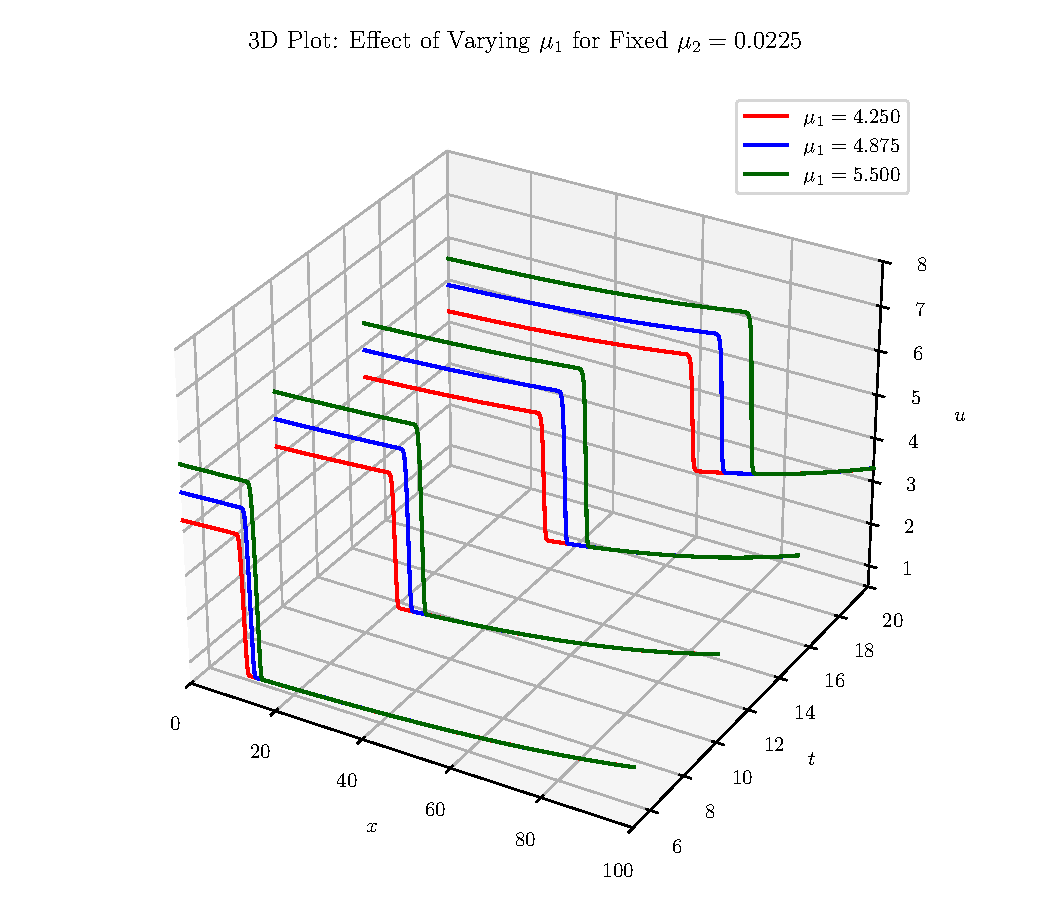
\includegraphics[width=0.45\textwidth]{Figures/plot_mu1_variation.pdf}
    \hfill
    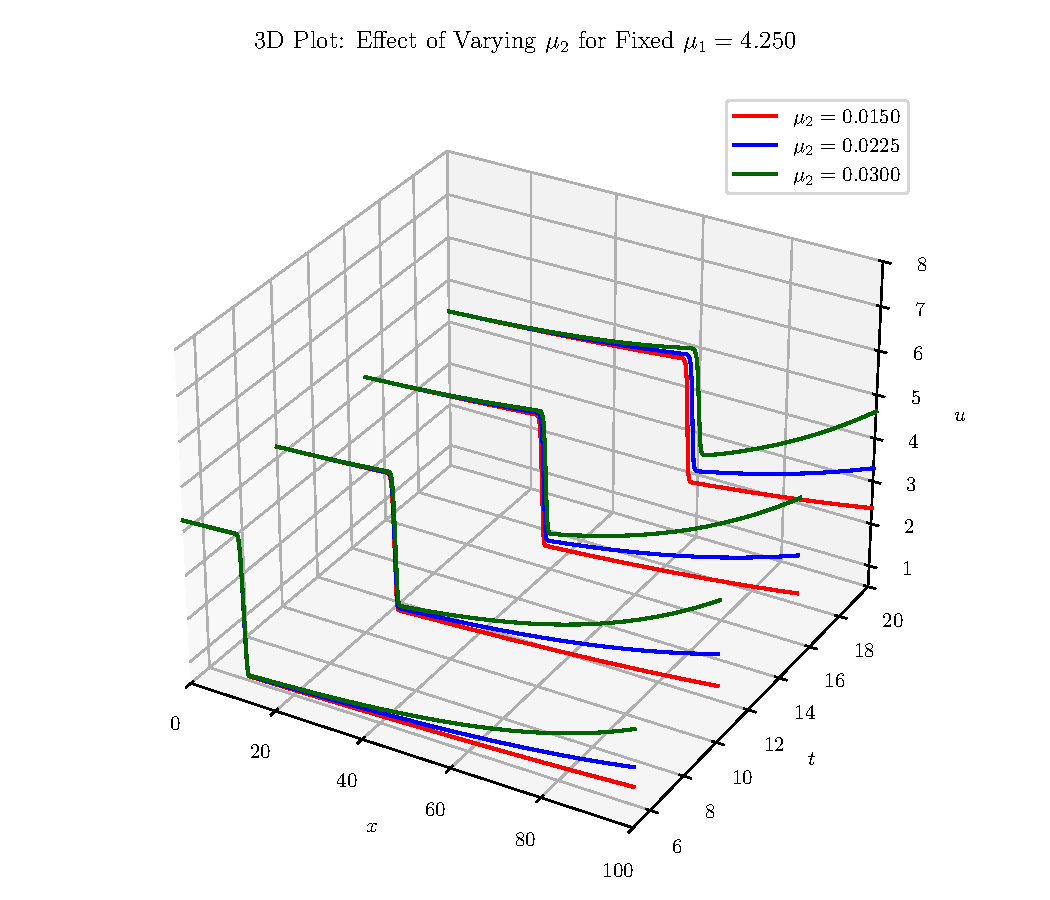
\includegraphics[width=0.45\textwidth]{Figures/plot_mu2_variation.pdf}
    \caption{3D plots of the full-order solution \(u(x,t)\). \textbf{Left:} Varying \(\mu_1 \in \{4.250, 4.875, 5.500\}\) with fixed \(\mu_2 = 0.0225\). \textbf{Right:} Varying \(\mu_2 \in \{0.0150, 0.0225, 0.0300\}\) with fixed \(\mu_1 = 4.875\).}
    \label{fig:3d_parametric}
\end{figure}

\begin{figure}[htbp]
    \centering
    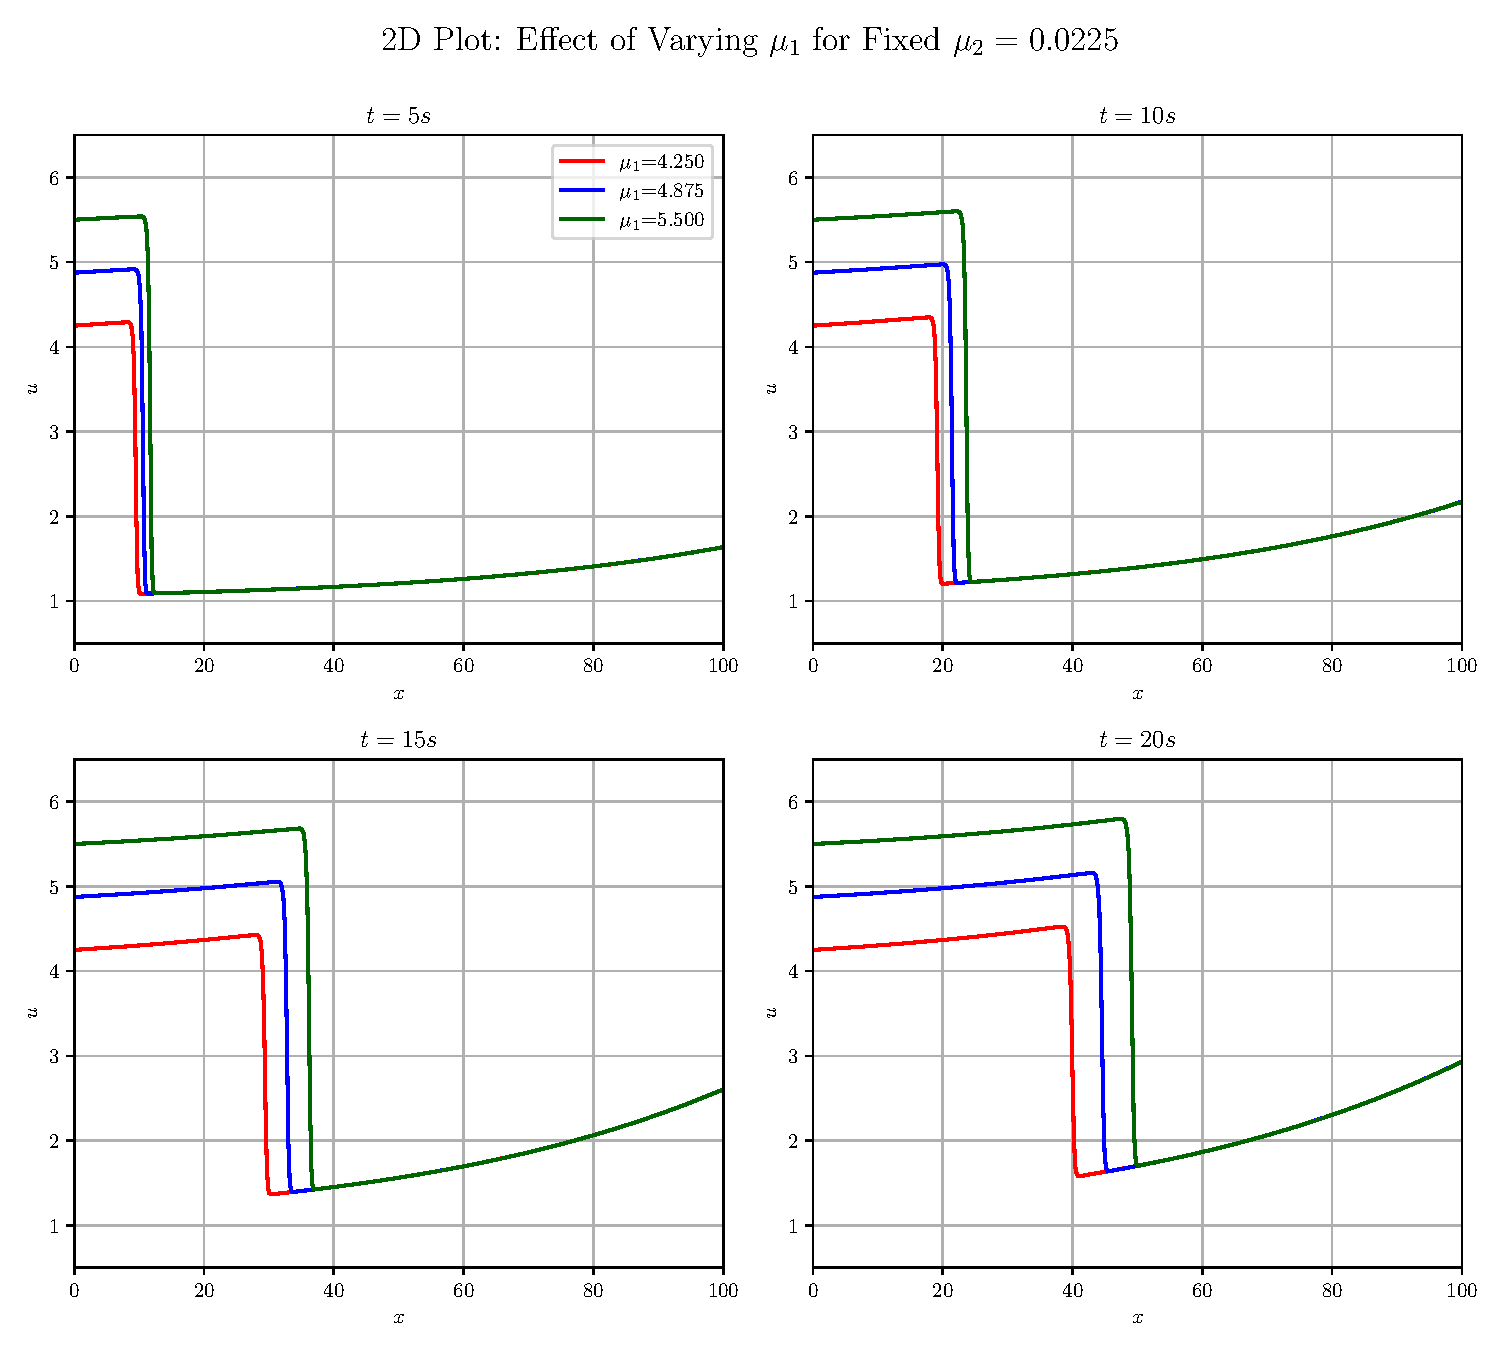
\includegraphics[width=0.65\textwidth]{Figures/subplot_mu1_variation.pdf}
    \caption{2D time-slice profiles at \(t = \{5,10,15,20\}\) seconds for different \(\mu_1\) values, with \(\mu_2 = 0.0225\) fixed.}
    \label{fig:subplots_mu1_fixed_mu2}
\end{figure}

\begin{figure}[htbp]
    \centering
    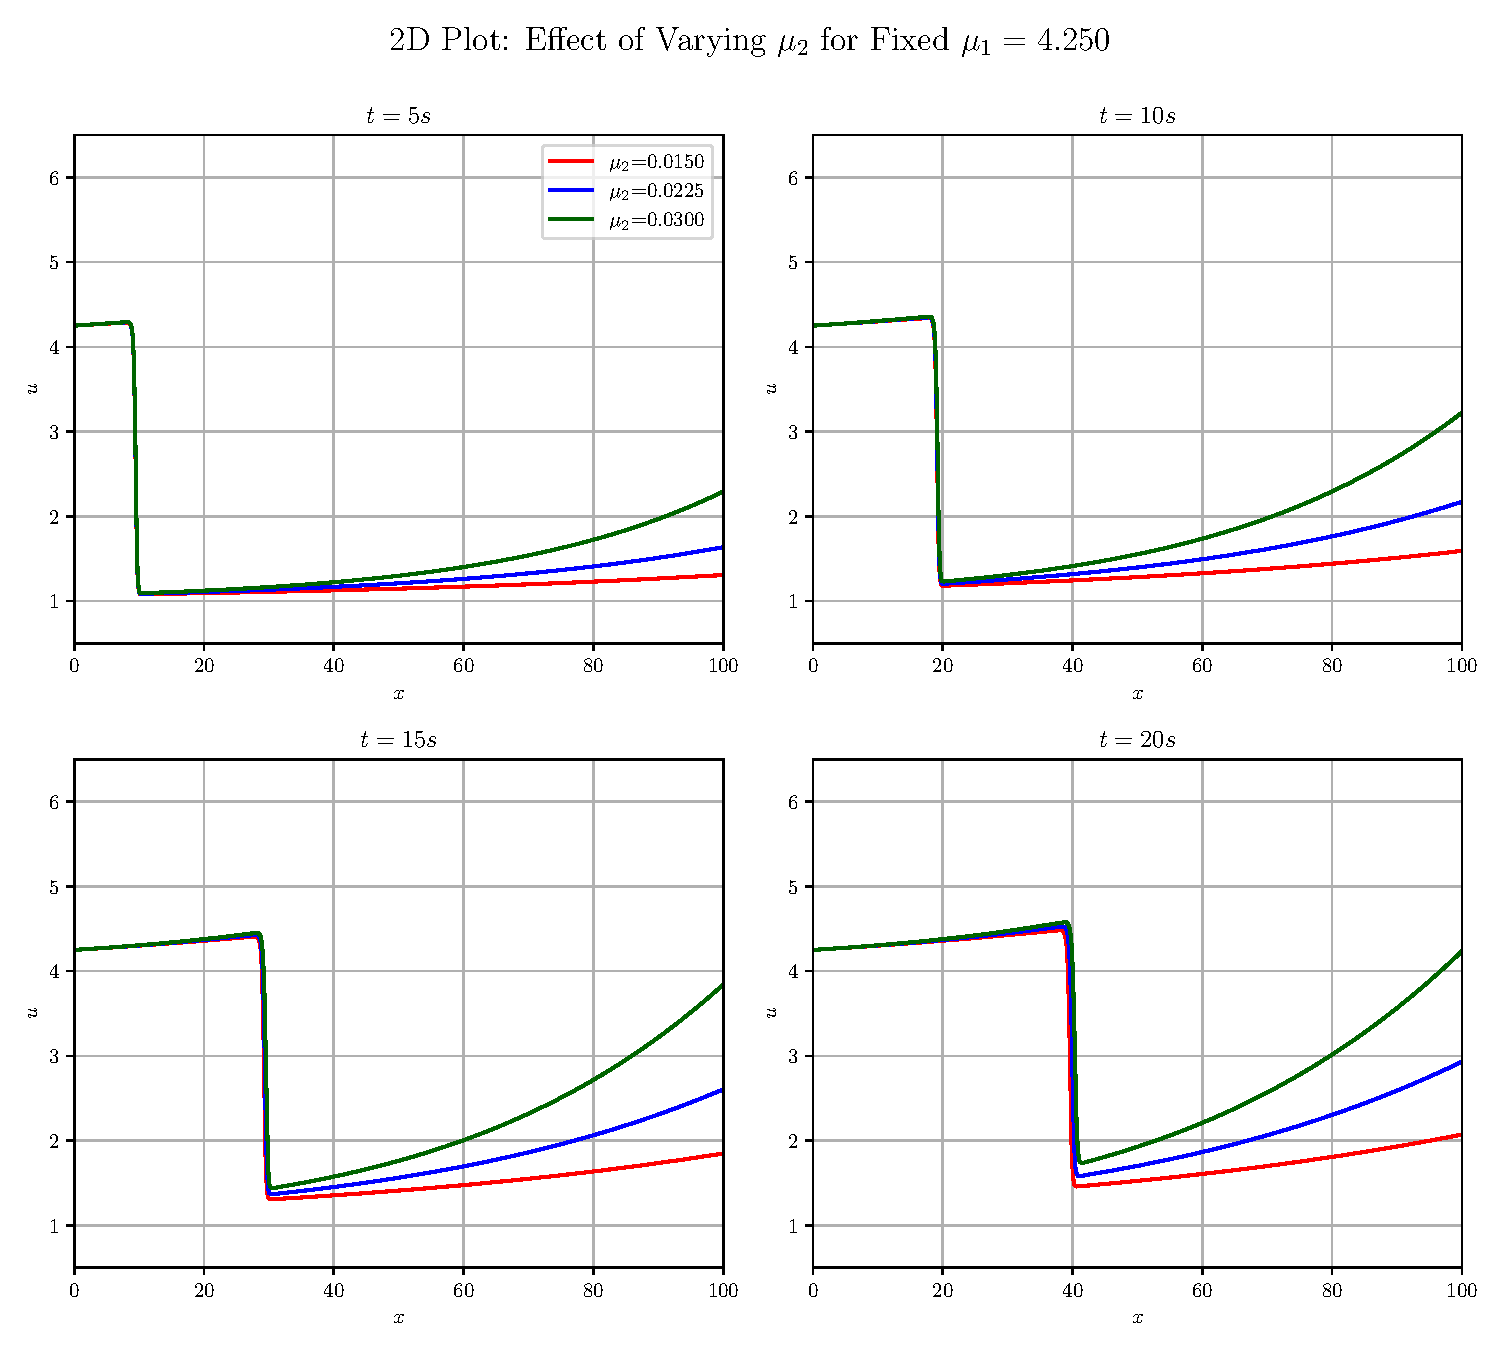
\includegraphics[width=0.65\textwidth]{Figures/subplot_mu2_variation.pdf}
    \caption{2D time-slice profiles at \(t = \{5,10,15,20\}\) seconds for different \(\mu_2\) values, with \(\mu_1 = 4.875\) fixed.}
    \label{fig:subplots_mu2_fixed_mu1}
\end{figure}

Since full 3D or multi-panel 2D visualizations are impractical for repeated comparison, Figure~\ref{fig:overlay_mu1_4875_mu2_0225} provides a compact view of the solution evolution by overlaying selected time instants for a representative parameter configuration. This will serve as a reference for subsequent comparisons across discretization methods and reduced-order approximations.

\begin{figure}[htbp]
    \centering
    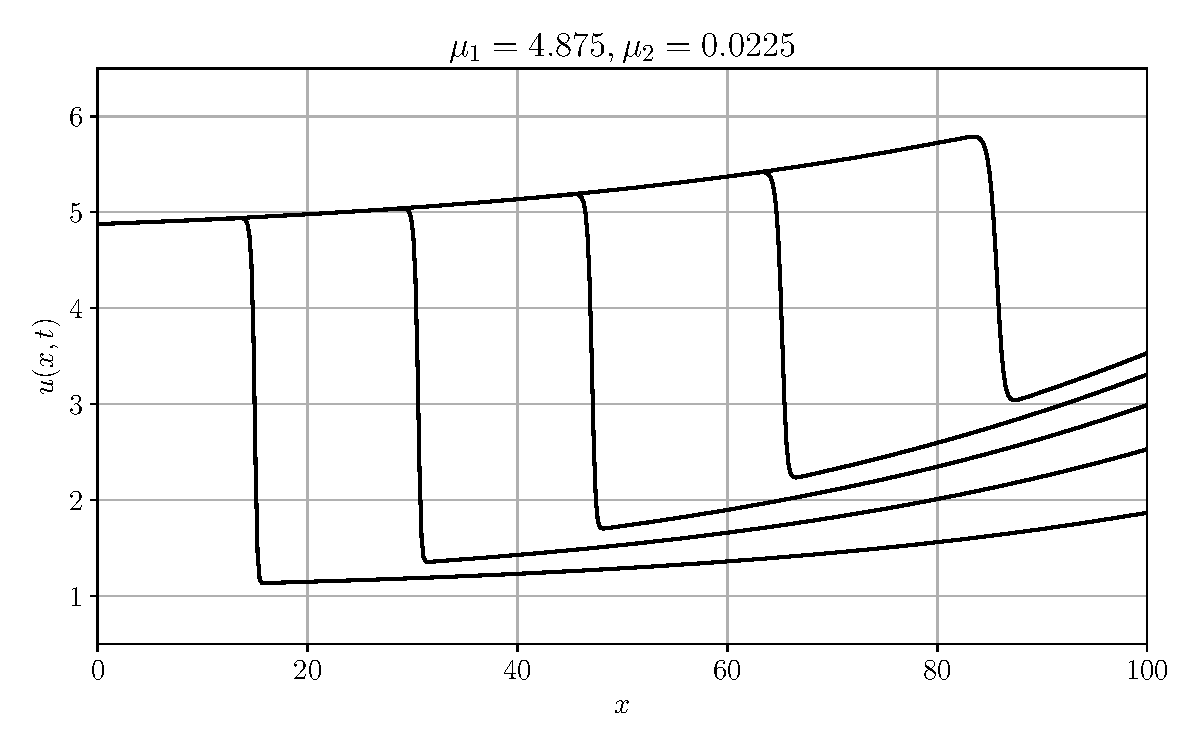
\includegraphics[width=0.7\textwidth]{Figures/overlayed_fom_mu1_4.875_mu2_0.0225.pdf}
    \caption{
    Overlay of the velocity field \( u(x,t) \) at several time instants for parameter configuration \( \bm{\mu} = [4.875,\; 0.0225] \). 
    The selected snapshots illustrate the evolution of the nonlinear wave profile at \( t = 5,\,10,\,15,\,20,\,25\,\text{s} \). 
    This compact visualization is used to qualitatively assess solution features such as steepening fronts and overall transport behavior. 
    Labels are omitted to keep the plot clean for later comparisons between discretization strategies and reduced-order models.
    }
    \label{fig:overlay_mu1_4875_mu2_0225}
\end{figure}

\subsection{Comparison across discretization methods}

To validate the finite element formulation introduced in this chapter and to benchmark its performance, its results are compared against two alternative discretization strategies: finite volume and finite difference. These additional implementations are described in detail in Appendices~\ref{appendix:fvm_burgers} and~\ref{appendix:fd_burgers}, respectively.

The comparison is conducted for two representative parameter configurations:
\begin{itemize}
    \item \(\bm{\mu}_\text{A} = [4.250,\; 0.0150]\): low inflow and mild source;
    \item \(\bm{\mu}_\text{B} = [5.500,\; 0.0300]\): high inflow and steep source.
\end{itemize}

Figure~\ref{fig:discretization_comparison_muA} and Figure~\ref{fig:discretization_comparison_muB} present overlayed plots of the velocity field at selected time instants for each method. In all cases, the same initial and boundary conditions, source term, and time stepping scheme are used to ensure a fair comparison.

Overall, the three methods exhibit excellent qualitative agreement in wave propagation and steepening behavior. Minor differences are observed in the sharpness of the wave front and dissipation characteristics. These discrepancies can be attributed to differences in numerical diffusion, order of accuracy, and stabilization mechanisms inherent to each scheme.

For the remainder of this chapter, the finite element method is adopted as the baseline discretization for the model problem. This choice is motivated by its alignment with the Kratos Multiphysics framework, which supports the broader reduced-order modeling developments presented in the thesis. Nevertheless, the finite difference implementation proved invaluable during early-stage algorithmic development and testing due to its simplicity and flexibility. Furthermore, the finite volume is revisited in Chapter~\ref{chap:article4}, where it is employed in the context of nonlinear subspace reduced-order models through its integration with the AERO-F platform.

\begin{figure}[htbp]
    \centering
    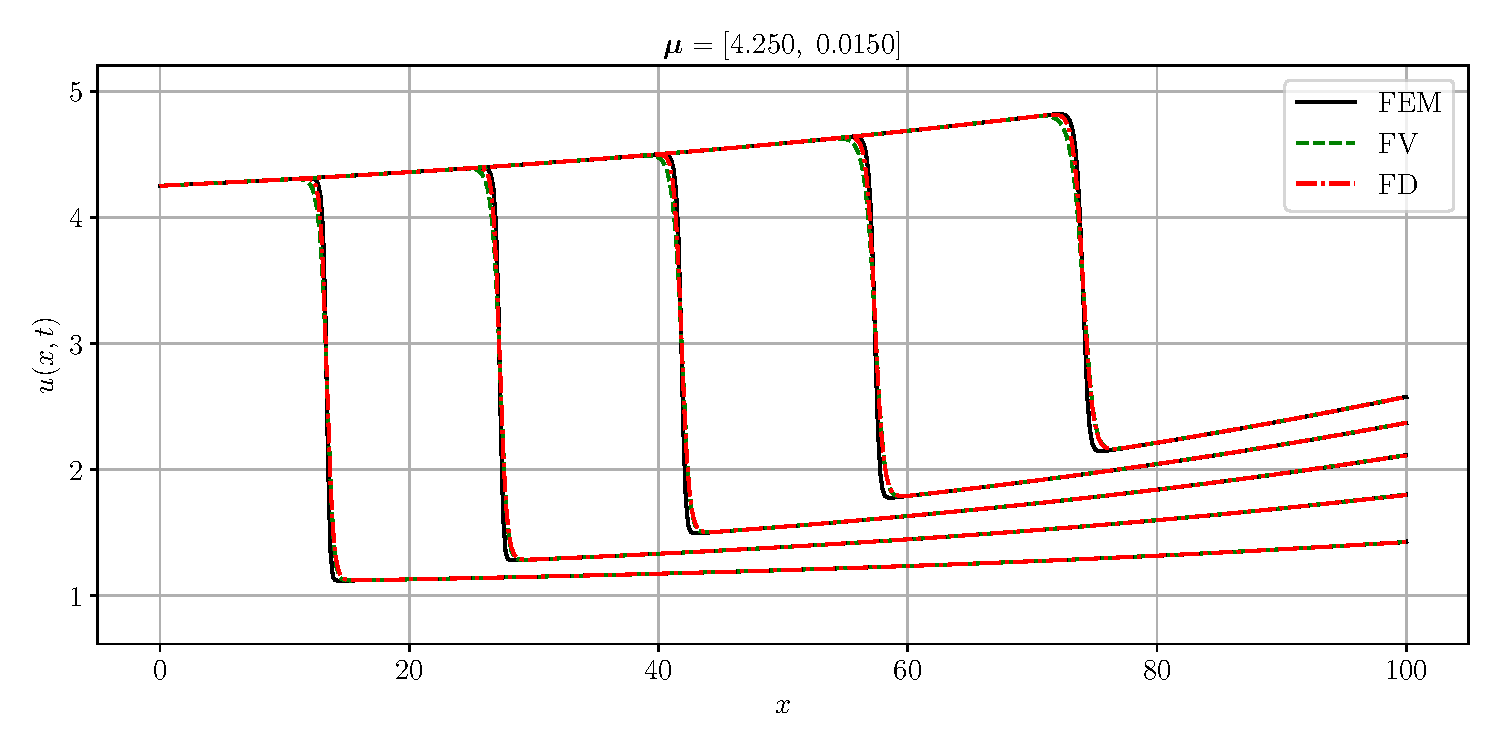
\includegraphics[width=0.7\textwidth]{Figures/discretization_comparison_overlay_mu1_4.250_mu2_0.0150.pdf}
    \caption{
    Comparison of FEM, FV, and FD results for parameter configuration \(\bm{\mu}_\text{A} = [4.250,\; 0.0150]\).
    The figure shows overlayed velocity profiles at multiple time instants.
    All methods produce consistent solutions, with minor variations in wave steepness and dissipation due to numerical differences.
    }
    \label{fig:discretization_comparison_muA}
\end{figure}

\begin{figure}[htbp]
    \centering
    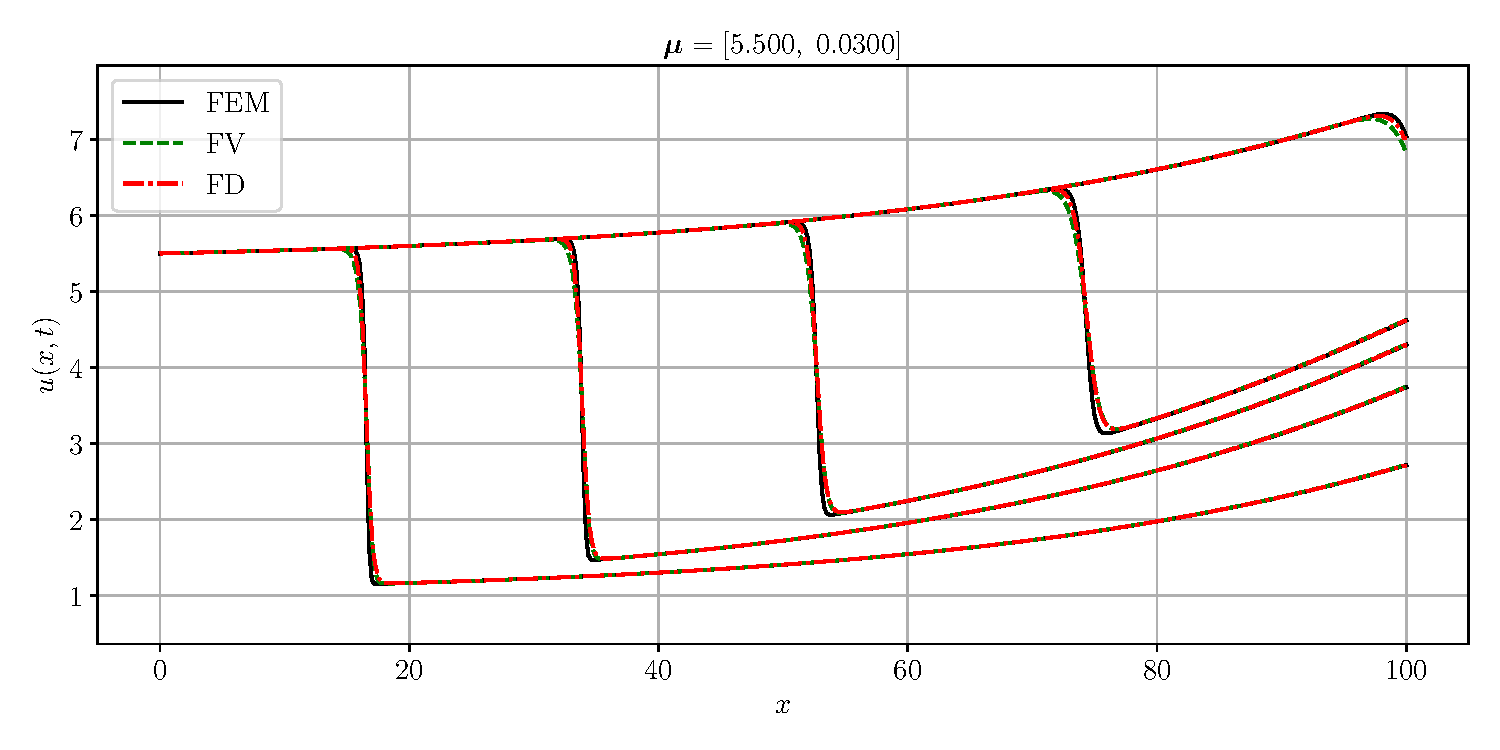
\includegraphics[width=0.7\textwidth]{Figures/discretization_comparison_overlay_mu1_5.500_mu2_0.0300.pdf}
    \caption{
    Comparison of FEM, FV, and FD results for parameter configuration \(\bm{\mu}_\text{B} = [5.500,\; 0.0300]\).
    The figure reveals sharper gradients and nonlinear transport effects.
    The agreement between methods supports the fidelity of the implemented solvers.
    }
    \label{fig:discretization_comparison_muB}
\end{figure}

\paragraph{Toward a unified reduced formulation.}
Equations~\eqref{eq:residual_fem}, \eqref{eq:residual_fv}, and \eqref{eq:residual_fd_vector} show that, irrespective of whether the governing equations are discretised by finite elements, finite volumes, or finite differences, the fully discrete problem always reduces to solving a nonlinear residual equation of the generic form
\begin{equation}
\mathbf{R}(\mathbf{u}) = \boldsymbol{0}.
\label{eq:general_residual}
\end{equation}
Here \(\mathbf{u}\) denotes the discrete state vector and \(\mathbf{R}\) the associated residual operator; the suppressed dependences on the time level and the parameter vector \(\boldsymbol{\mu}\) will be introduced in the following chapters.  

The focus of the remainder of this thesis is to develop projection‑based reduced‑order models that operate directly on~\eqref{eq:general_residual}, replacing the large‑scale system with a much smaller one while preserving accuracy for all three underlying discretisations.  Chapter~\ref{chap:linear_prom} begins this programme by constructing linear subspace models (also introducing the notion of hyper‑reduction techniques) that minimise the discrete residual in a reduced coordinate space; subsequent chapters extend the framework for nonlinear reduction.


% \clearpage

% \section*{Nomenclature}

% \begin{tabular}{ll}
% FEM                    & Finite Element Method \\
% SUPG                   & Streamline-Upwind/Petrov--Galerkin stabilization \\
% $u(x,t)$               & Velocity field (scalar continuous) \\
% $\mathbf{u}$           & Vector of nodal unknowns (discrete velocity field) \\
% $v(x)$                 & Test function (scalar) \\
% $f(x,t)$               & Source term (scalar continuous) \\
% $L$                    & Spatial domain length \\
% $T$                    & Final simulation time \\
% $\mu_1$                & Dirichlet inflow boundary condition parameter \\
% $\mu_2$                & Source term parameter \\
% $N_e$                  & Number of finite elements \\
% $N$                    & Number of nodes (degrees of freedom) \\
% $N_j(x)$               & Finite element shape function (scalar) \\
% $\mathbf{M}$           & Mass matrix \\
% $\mathbf{C}(\mathbf{u})$ & Nonlinear convection matrix/operator \\
% $\mathbf{S}(\mathbf{u})$ & SUPG stabilization vector/operator \\
% $\mathbf{F}(t)$        & Load vector \\
% $\Delta t$             & Time step size \\
% $\mathbf{R}(\mathbf{u})$ & Nonlinear residual vector \\
% $\mathbf{J}(\mathbf{u})$ & Jacobian matrix of the residual \\
% \end{tabular}

